For both the cube and the single axis setup, the system dynamics can be analyzed in one plane only, provided the reaction wheel is parallel to that plane. In that case, the system is effectively an inverted pendulum constrained to one axis around a pivot point. When doing the mathematical analysis, we focused on the single axis setup as in Figure~\ref{fig:cubli_planar_diagram},

\begin{figure}[H]
    \centering
    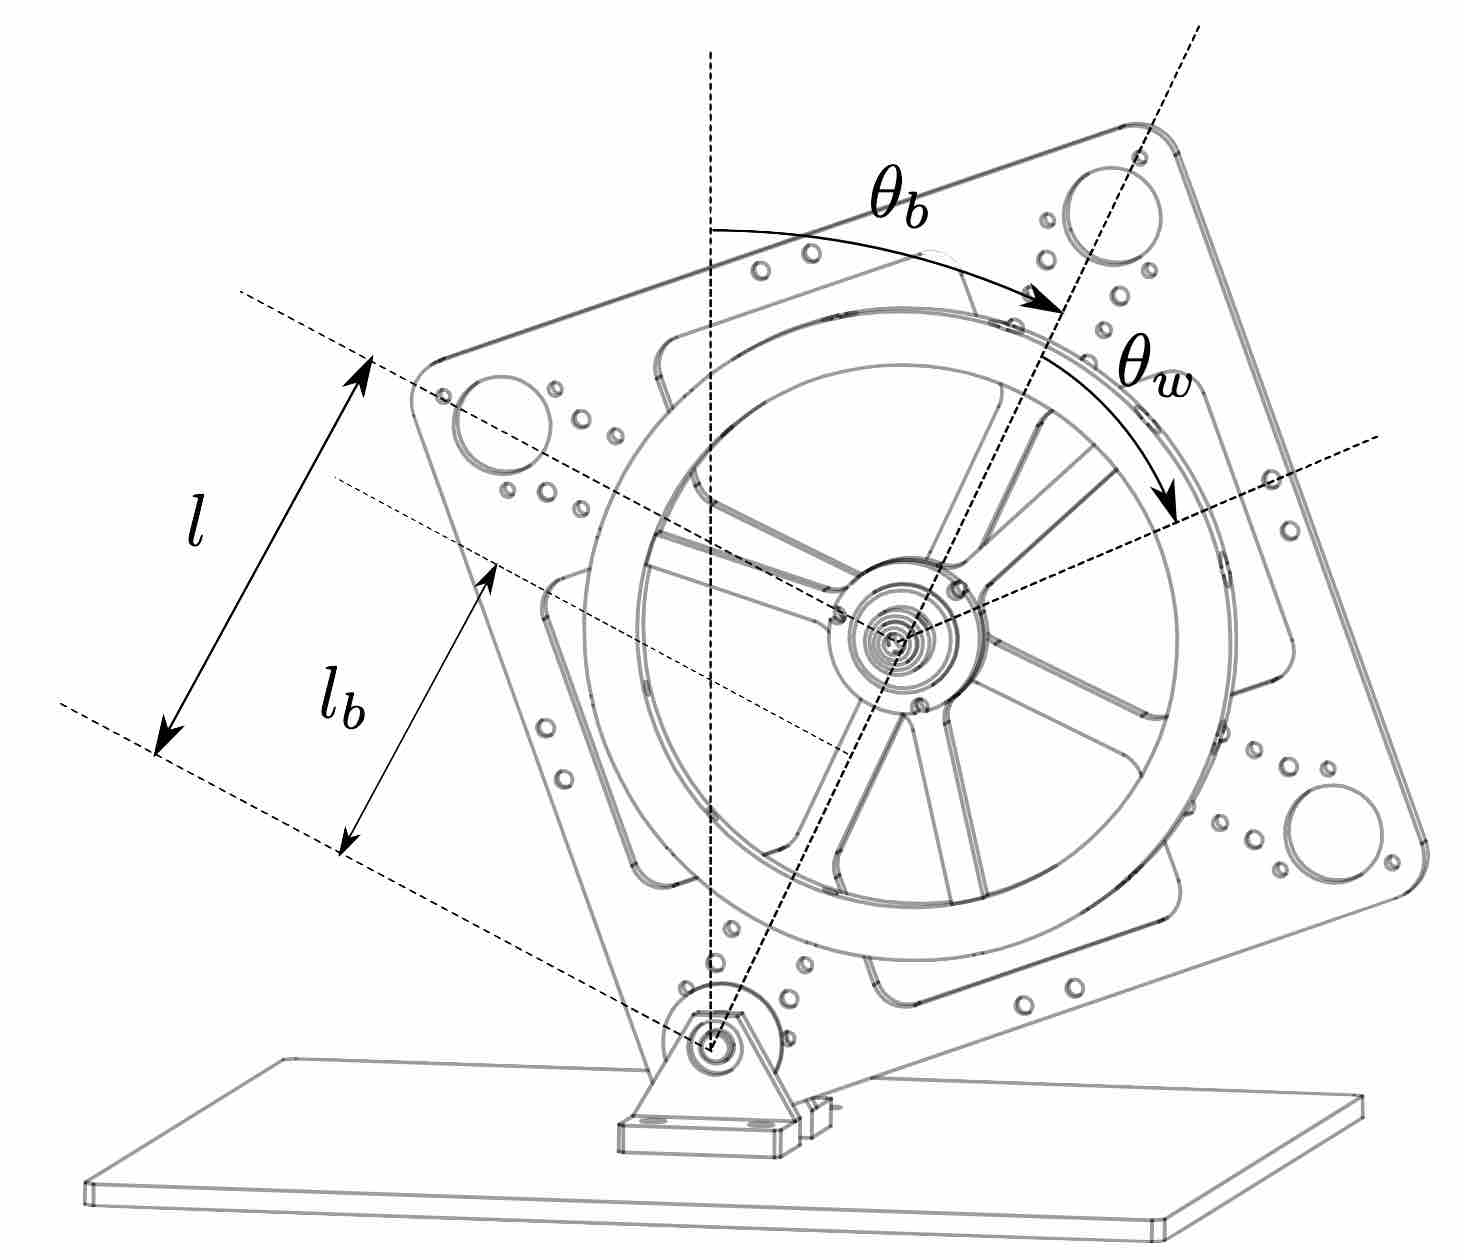
\includegraphics[width=.8\linewidth]{figures/Planar-diagram.jpg}
    \caption{Diagram of single axis setup from \cite{cubli-planar}.}
    \label{fig:cubli_planar_diagram}
\end{figure}

\noindent
where $\theta_b$ is the tilt angle of the pendulum body and $\theta_w$ is the angle of the wheel with respect to the body. The distance between the motor and the pivot point $O$ is denoted by $l$ whereas $l_b$ is the distance between the pendulum body's center of mass and $O$. Due to the symmetry of our prototype we assumed that $l = l_b$. We also assumed zero friction in the pivot point due to the use of a ball bearing. With these assumptions, we can modify the system of equations from \cite{cubli-planar} to get

\begin{equation}\label{eq:system}
    \begin{gathered}
        \ddot\theta_b = \frac{(m_b + m_w)gl\sin\theta_b - T_m +C_w\dot\theta_w}{I_b + m_wl^2}, \\
        \ddot\theta_w = \frac{(I_b + I_w + m_wl^2) \left( T_m - C_w\dot\theta_w \right)}{I_w(I_b + m_wl^2)} \\- \frac{(m_b + m_w)gl\sin\theta_b}{I_b + m_wl^2},
    \end{gathered}
\end{equation}

\noindent
where $m_b$ is the mass of the structure and the motor, $m_w$ is the mass of the reaction wheel, $T_m$ is the motor torque, $C_w$ is the dynamic friction coefficient of the wheel. $I_w$, $I_b$ are the moments of inertia of the wheel around its rotational axis and the pendulum body around $O$ respectively.

\subsection{Motor dynamics}
The motors used were initially simple brushed DC motors whose relation between torque $T_m$ and current $i$ drawn by the motor can be described as

\begin{equation}
    T_m = K_mi,
\end{equation}

\noindent
where $K_m$ is the torque constant. We can hence describe the acceleration of the reaction wheel as

\begin{equation}\label{eq:motor}
    \ddot\theta_w = \frac{K_m i - C_w\dot\theta_w}{I_w}.
\end{equation}

\subsection{State-space model}
We can now combine \eqref{eq:system} and \eqref{eq:motor} to get a full model that accounts for the current $i$. By using the approximation of small angles, $\sin\theta \approx \theta$, the system of equations becomes linear. The state variables are chosen as $\mathbf{x} = [\theta_b \ \dot\theta_b \ \dot\theta_w]^T$. Linearizing around $[0 \ 0 \ 0]^T$ gives

\begin{equation}\label{eq:state-space}  
    \begin{gathered}
        \dot{\mathbf{x}} = A\mathbf{x} + Bu, \\
        \mathbf{y} = C\mathbf{x},
    \end{gathered}
\end{equation}

\noindent
where

\begin{equation}\label{eq:ss-matrices}
    \begin{gathered}
        A =
        \begin{bmatrix}
            0 & 1 & 0 \\
            \frac{(m_b+m_w)gl}{I_b+m_wl^2} & 0 & \frac{C_w}{I_b+m_wl^2} \\
            -\frac{(m_b+m_w)gl}{I_b+m_wl^2} & 0 & -\frac{C_w(I_b+I_w+m_wl^2)}{I_w(I_b+m_wl^2)}
        \end{bmatrix}
        , \\
        B =
        \begin{bmatrix}
            0 \\
            -\frac{K_m}{I_b + m_wl^2} \\
            \frac{K_m(I_b+I_w+m_wl^2)}{I_w(I_b+m_wl^2)}
        \end{bmatrix}
        \text{ and } C =
        \begin{bmatrix}
            1 & 0 & 0 \\
            0 & 1 & 0 
        \end{bmatrix},
    \end{gathered}
\end{equation}

\noindent
where the control signal $u$ is the current $i$ and the output signal $\mathbf{y}$ is both $\theta_b$ and $\dot\theta_b$. The goal is to control only $\theta_b$ and stabilize it around 0, but the angular velocity $\dot\theta_b$ will also be directly readable from sensor data.
\\\\
The state-space model was then discretized using zero-order hold to get the discrete-time model

\begin{equation}\label{eq:ss-disc}
    \begin{gathered}
        \mathbf{x}_{k+1} = A_d\mathbf{x}_k + B_du_k,\\
        \mathbf{y}_k = C\mathbf{x}_k,
    \end{gathered}
\end{equation}

\noindent
where $A_d$ and $B_d$ are the discrete-time counterparts to $A$ and $B$.

\subsection{Parameter identification}
To simulate the state-space model, the physical parameters had to be identified. $I_b$ was calculated with

\begin{equation}\label{eq:Ib}
    I_{b} = \frac{s_{f}^2}{6}m_{f} + \frac{r_{m}^2}{2}m_{m} + (m_{f} + m_{m})l^2,
\end{equation}

\noindent
where $s_{f}$ is the side length of the frame, $r_{m}$ is the radius of the motor, $m_{f}$ is the mass of the frame and $m_{m}$ is the mass of the motor. $I_w$ was calculated with

\begin{equation}\label{eq:Iw}
    I_{w} = \frac{1}{2}m_{w}(r_{\text{outer}}+r_{\text{inner}})^2
\end{equation}

\noindent
where $r_{\text{outer}}$ is the radius of the wheel and $r_{\text{inner}}$ is the radius to the inner edge of the wheel. The maximum torque of the motor can be found in \cite{motor-datasheet}. The torque constant $K_{m}$ can also be calculated from the data sheet, using the equation

\begin{equation}\label{eq:Km}
    K_{m} = \frac{T_{2} - T_{1}}{i_{2} - i_{1}},
\end{equation}

\noindent
where the torques $T_1, T_2$ and currents $i_1, i_2$ were chosen at two different points.
